% Topic from _Linear Algebra_ Jim Hefferon
%  http://joshua.smcvt.edu/linalg.html
%  2012-Feb-12
\topic{Magic Squares}
% \newcommand{\magicsquares}{\mathcal{M}}
\index{magic squares|(}
A Chinese legend tells the story of a  
flood by the Lo river.
The people offered sacrifices to appease the river.
Each time a turtle emerged, 
walked around the sacrifice, and returned to the river.
Fuh-Hi, % (2858-2738~BC)
the founder of Chinese civilization,
interpreted this to mean that
the river did not accepted the sacrifices.  
A child provided the answer by noticing 
that on its shell the turtle had what is today
called the pattern of Lo Shu (``river scroll'').
\begin{center}
  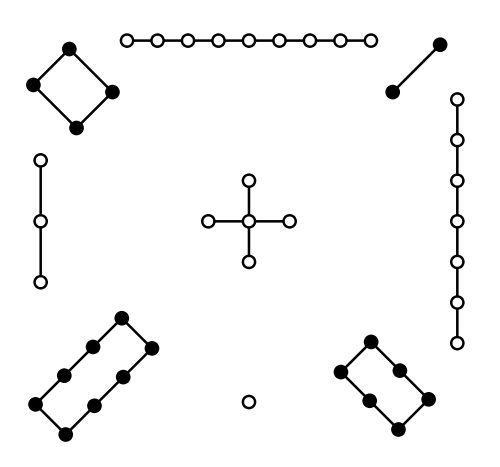
\includegraphics[height=1in]{LoShu.png}
\end{center}
The dots make a matrix.
\begin{center}
  \begin{tabular}{|c|c|c|}
    \hline
      $4$  &$9$  &$2$  \\ \hline
      $3$  &$5$  &$7$  \\ \hline
      $8$  &$1$  &$6$  \\ \hline    
  \end{tabular}
\end{center}
Each row, column, 
and diagonal adds to $15$
(the number of days in each of the twenty four cycles of the 
Chinese solar year).
Now that the people knew how much to sacrifice, at last the river's anger cooled.
% (http://en.wikipedia.org/wiki/Lo_Shu_Square)

A square matrix is 
\definend{magic}\index{magic square}\index{matrix!magic square}
if each row, column, and diagonal add to the same
value.
This value is the \definend{magic number}.

Another example of a magic square appears in the engraving
\textit{Melencolia I} by Albrecht D\"urer.
% (http://en.wikipedia.org/wiki/Melencolia_I)
\begin{center}
  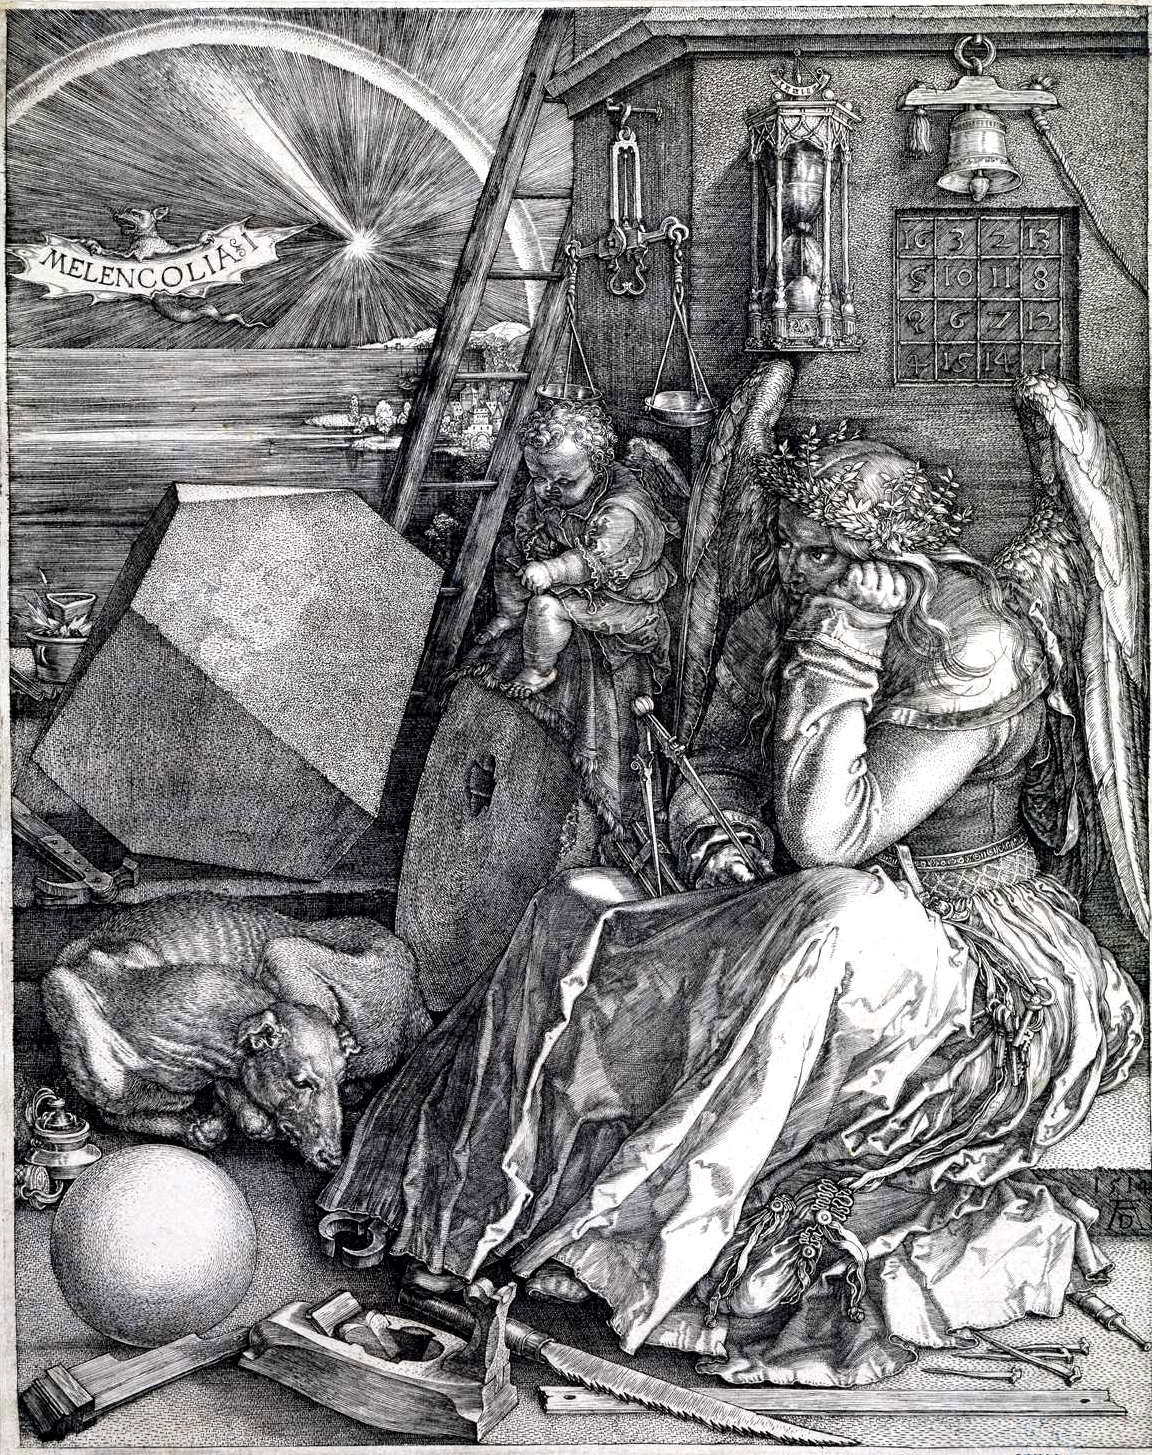
\includegraphics[height=2.25in]{Melencolia.jpg} % wikipedia http://upload.wikimedia.org/wikipedia/commons/1/14/Melencolia_I_%28Durero%29.jpg
\end{center}
One interpretation is that this depicts melancholy, a depressed state.
The figure, genius,
is surrounded by a wealth of fascinating things to be explored.
These include
the compass, the geometrical solid, the scale, and the hourglass.
But the figure is unmoved; all the things are unused.
One of the potential delights is the $\nbyn{4}$ matrix in the upper right.
The rows, columns, and diagonals add to $34$.
\begin{center}
  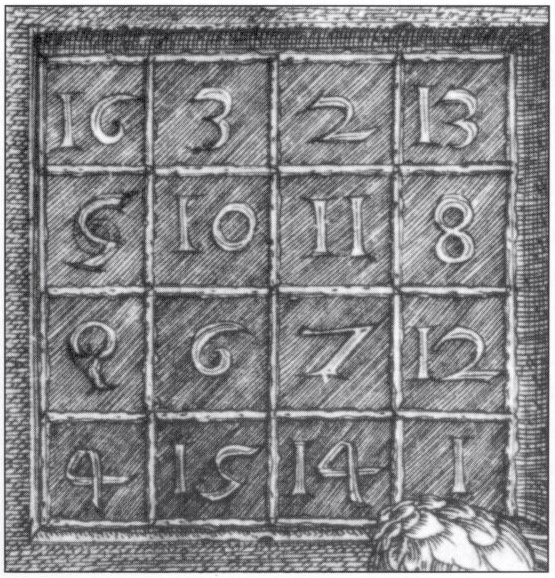
\includegraphics[height=1.25in]{Melencoliadetail.jpg} % wikipedia http://upload.wikimedia.org/wikipedia/commons/7/7e/Albrecht_D%C3%BCrer_-_Melencolia_I_%28detail%29.jpg
  \qquad
  \begin{tabular}[b]{|c|c|c|c|}
    \hline
      $16$  &$3$  &$2$  &$13$  \\ \hline
      $5$   &$10$ &$11$ &$8$   \\ \hline
      $9$   &$6$  &$7$  &$12$  \\ \hline    
      $4$   &$15$ &$14$ &$1$  \\ \hline    
  \end{tabular}
\end{center}
The middle entries on the bottom row give $1514$, the 
date of the engraving.

A sum of two same-sized magic squares is magic and a 
scalar multiple of a magic square is magic, so the set of 
$\nbyn{n}$ magic squares
$\magicsquares_n$ is a subspace of $\matspace_{\nbyn{n}}$.

The set $\magicsquares_{n,0}$ of $\nbyn{n}$~magic squares with magic number~$0$ 
is another subspace.

Every $\nbyn{1}$ square is magic, trivially.
If the rows, columns, and diagonals of a $\nbyn{2}$ matrix add to $k$
\begin{equation*}
  \begin{mat}
    a  &b  \\
    c  &d
  \end{mat}
\end{equation*}
then $a+b=s$, $c+d=s$, $a+c=s$, $b+d=s$, $a+d=s$, and $b+c=s$.
\nearbyexercise{exer:TwoByTwoMagicSqUnique} shows that
the system has the unique solution $a=b=c=d=s/2$.
So $\magicsquares_2$ is a one-dimensional subspace of $\matspace_{\nbyn{2}}$.
In this Topic we will show that for $n>2$ the 
dimension of
$\magicsquares_n$ is $n^2-n$.

A square matrix is \definend{semimagic} if 
the rows and columns add to the same value (that is, we drop the
condition on the diagonals).
The set of semimagic squares $\mathcal{H}_n$ 
is a subspace of $\matspace_{\nbyn{n}}$.
So is the set $\mathcal{H}_{n,0}$  
of $\nbyn{n}$~semimagic squares with magic number~$0$. 
We start by showing that this space has dimension $(n-1)^2$.

The sum of numbers down the upper-left to lower-right diagonal
$\trace (M)=m_{1,1}+\cdots+m_{n,n}$ is the 
\definend{trace}\index{trace}\index{matrix!trace}
of the matrix~$M$.
We define also the sum down the other diagonal
$\trace^* (M)=m_{1,n}+\cdots+m_{n,1}$.
Consider the map $\map{\theta}{\mathcal{H}_n}{\Re^2}$ that sends a 
matrix~$M$ to
the ordered pair $(\trace(M),\trace^*(M))$.
\nearbyexercise{xx} shows that this function is linear. 
and that its nullspace is the space $\magicsquares_{n,0}$
of $\nbyn{n}$ magic squares with magic number~$0$.

We will show that $\theta$ is an onto map when $n\geq 3$.
Because $\theta$ is linear we need only find a basis for $\Re^2$ that is the
image of two members of $\mathcal{H}_n$.
Consider the matrix $C\in \mathcal{H}_n$ that has all entries zero except
that the four corners are $c_{1,1}=c_{n,n}=1$ and $c_{1,n}=c_{n,1}=-1$.
Also consider the matrix $D\in \mathcal{H}_n$ with all entries zero except that 
$d_{1,1}=d_{2,2}=1$ and $d_{1,2}=d_{2,1}=-1$.
We have
\begin{equation*}
  \theta(C)=\colvec{2 \\ -2}
  \qquad
  \theta(D)=\begin{cases}
               \colvec{2 \\ -1}  &\text{if $n=3$}  \\
               \colvec{2 \\  0}  &\text{if $n>3$}
            \end{cases}
\end{equation*}
and so the image of $\theta$ includes a basis for $\Re^3$.
Thus $\theta$ is onto.

Theorem~Two.II.\ref{th:RankPlusNullEqDim} says that for any linear map the
dimension of the domain equals its rank plus its nullity.
Here that gives $\dim(\mathcal{H}_n)=\dim(\magicsquares_{n,0})+2 $

% It is an unsolved problem to determine the number of magic squares of an arbitrary order, but the number of distinct magic squares (excluding those obtained by rotation and reflection) of order n=1, 2, ... are 1, 0, 1, 880, 275305224, ... (Sloane's A006052; Madachy 1979, p. 87). The 880 squares of order four were enumerated by Frénicle de Bessy in 1693, and are illustrated in Berlekamp et al. (1982, pp. 778-783). The number of 5×5 magic squares was computed by R. Schroeppel in 1973. The number of 6×6 squares is not known, but Pinn and Wieczerkowski (1998) estimated it to be (1.7745+/-0.0016)×10^(19) using Monte Carlo simulation and methods from statistical mechanics. 
%(http://mathworld.wolfram.com/MagicSquare.html)


\begin{exercises}
  \item \label{exer:TwoByTwoMagicSqUnique}
    Solve the system $a+b=s$, $c+d=s$, $a+c=s$, $b+d=s$, $a+d=s$, and $b+c=s$.
    \begin{answer}
      For any $k$ we have this.
      \begin{equation*}
        \begin{amat}{4}
          1  &1  &0  &0  &s  \\
          0  &0  &1  &1  &s  \\
          1  &0  &1  &0  &s  \\
          0  &1  &0  &1  &s  \\
          1  &0  &0  &1  &s  \\
          0  &1  &1  &0  &s            
        \end{amat}\;\grstep[-\rho_1+\rho_5]{-\rho_1+\rho_3}\;
        \begin{amat}{4}
          1  &1  &0  &0  &s  \\
          0  &0  &1  &1  &s  \\
          0  &-1 &1  &0  &0  \\
          0  &1  &0  &1  &s  \\
          0  &-1 &0  &1  &0  \\
          0  &1  &1  &0  &s            
        \end{amat}\;\grstep{-\rho_2\leftrightarrow\rho_6}\;
        \begin{amat}{4}
          1  &1  &0  &0  &s  \\
          0  &1  &1  &0  &s  \\          
          0  &-1 &1  &0  &0  \\
          0  &1  &0  &1  &s  \\
          0  &-1 &0  &1  &0  \\
          0  &0  &1  &1  &s  
        \end{amat}\;\grstep[-\rho_2+\rho_4 \\ \rho_2+\rho_5]{-\rho_2+\rho_3}\;
        \begin{amat}{4}
          1  &1  &0  &0  &s  \\
          0  &1  &1  &0  &s  \\          
          0  &0  &2  &0  &s  \\
          0  &1  &-1 &1  &0  \\
          0  &0  &1  &1  &s  \\
          0  &0  &1  &1  &s  
        \end{amat}
      \end{equation*}
      The unique solution is $a=b=c=d=s/2$.
    \end{answer}
  \item Let $M$ be a $\nbyn{3}$ magic square with magic number~$s$.
    \begin{exparts}
      \partsitem Prove that the sum of $M$'s entries is $3s$.
      \partsitem Prove that $s=3\cdot m_{2,2}$.
      \partsitem Prove that $m_{2,2}$ is the average of the entries
        in its row, its column, and in each diagonal.
      \partsitem Prove that $m_{2,2}$ is the median of $M$'s entries.
    \end{exparts}
    \begin{answer}
      \begin{exparts}
        \partsitem The sum of the entries of $M$ is the sum of the sums of
          the three rows. 
        \partsitem The constraints on entries of $M$ involving the center 
          entry make this system.
          \begin{equation*}
            \begin{linsys}{3}
              m_{2,1}  &+  &m_{2,2}  &+  &m_{2,3}  &=  &s  \\ 
              m_{1,2}  &+  &m_{2,2}  &+  &m_{3,2}  &=  &s  \\ 
              m_{1,1}  &+  &m_{2,2}  &+  &m_{3,3}  &=  &s  \\ 
              m_{1,3}  &+  &m_{2,2}  &+  &m_{3,1}  &=  &s  
            \end{linsys}
          \end{equation*}
          Adding those four equations counts each matrix entry once and only
          once, except that the center entry is counted four times.
          Thus the left side sums to $3s+3m_{2,2}$ while the right sums to $4s$.
          So $3m_{2,2}=s$.
        \partsitem
          The second row adds to $s$ so $m_{2,1}+m_{2,2}+m_{2,3}=3m_{2,2}$,
          giving that $(1/2)\cdot(m_{2,1}+m_{2,3})=m_{2,2}$.
          The same goes for the column and the diagonals.
        \partsitem
          By the prior exercise either both $m_{2,1}$ and $m_{2,3}$ are equal
          to $m_{2,2}$ or else one is greater while one is smaller.
          Thus $m_{2,2}$ is the median of the set
          $\set{m_{2,1},m_{2,2},m_{2,3}}$.
          The same reasoning applied to the second column shows that 
          Thus $m_{2,2}$ is the median of the set
          $\set{m_{1,2},m_{2,1},m_{2,2},m_{2,3},m_{3,2}}$.
          Extending to the two diagonals shows it is the median of the set
          of all entries.
      \end{exparts}
    \end{answer}
        

\end{exercises}
\index{magic squares|)}
\endinput


